\documentclass{lncs-template/llncs}

\usepackage{graphicx}
% \usepackage[all]{xy}
% \usepackage{color}
% \usepackage{euscript}
% \usepackage[noend]{algpseudocode}
% \usepackage{algorithm}
% \usepackage{epsfig}
% \usepackage[all]{xy}
% \usepackage{subfigure}
% \usepackage{multirow}

\begin{document}

\title{Context-Based Ontology for Urban Data Integration}

\author{Michal Med\inst{1} and Petr K\v{r}emen\inst{2}}
\institute{
  Czech Technical University in Prague, Czech Republic\\ TODO@fel.cvut.cz \and 
  Department of Cybernetics, Faculty of Electrical Engineering, Czech Technical University in Prague, Czech Republic\\ \texttt{petr.kremen@fel.cvut.cz}
}

\maketitle

\begin{abstract}
Urban planning data are of big importance to both general public and domain experts like civil engineers, architects or urban planning specialists. Typically, the data are scattered within many datasets containing both geographical knowledge and taxonomical knowledge. The distributed nature of such data, as well as their complexity practically prevents formulating relevant geographic queries over multiple datasets. 

In this paper, we present a case study on ontology modeling of urban planning data of the City of Prague. We discuss the ontological nature of the domain, as well as formalization of the ontology in the OWL language. At the end of the paper we present various distributed queries over multiple datasets.
\end{abstract}

\section{Introduction}

Urban planning is a data-intensive domain encountering great interest of experts as well as of general public. Many data sources in urban planning are public by their nature, yet, different level of quality of the data sources, as well as their semantic heterogenity makes them difficult to interpret and exploit. Although ontologies for urban planning have been developed for over a decade (e.g. \cite{fonseca2000ontologies}, \cite{psyllidis2015ontology}), not much attention has been paid to the context-based knowledge representation in the domain. 

We came accross the need of context-sensitive ontology-based integration model during our research project aimed at integrating and exploiting urban data sources of the Prague Institute of Planning and Development (IPR). The institute has tens of datasets, content of which is typically visualized by means of a GIS. However, the integration of their content is missing. It turns out that many generic terms, like \emph{building}, \emph{construction}, or \emph{house}, are understood differently by architects, civil engineers, urban planning experts as well as general public. These semantic discrepancies have significant impact on subsequent data usage including statistics. Also, even a technique that would provide a limited set of datasets that would be necessary to explore manually in order to evaluate given query is missing.

Here we introduce a \emph{context-sensitive ontology-based model} of urban planning dataset integration. The model is based on the UFO ontology  \cite{guizzardi2005ontological} and its extensions by power types \cite{guizzardi2015powertypes}. The model is then formalized in an OWL~2 \cite{owl2-overview} ontology using SPARQL \cite{2013sparql}, resp. $SPARQL-DL^{NOT}$ \cite{Kremen:2012:EOQ:2607597.2607601} queries for distributed query formulation. The queries are discussed in terms of usability in the domain.

Section \ref{sec:bkg} presents the most important notions used in the paper.

% TODO paper organization

\section{Background}\label{sec:bkg} 

\subsection{Unified Foundational Ontology}

As a top-level ontology, we use the Unified Foundational Ontology (UFO). Comparing to other approaches (e.g. \cite{ggmos2002sod}, \cite{gs2009sstdso}, \cite{np2001tsuo}), it is an actively developed ontology that incorporates structural modeling, event modeling, mereology, as well as power types and context modeling. Furthemore, it provides an ontology design UML-based language OntoUML.

UFO consists of:
\begin{description}
 \item[UFO-A] is a foundational ontology analyzing structural modeling constructs \cite{g2006ofscm}, describing object types, taxonomies, associations and mereological relations,
 \item[UFO-B] is an ontology of events \cite{gwaga2013tofcme}, describing events and situations
 \item[UFO-C] is an ontology of social and intentional aspects \cite{gr2005bsao}, describing intentions and social aspects of agents, and
 \item[UFO-S] is an ontology of services \cite{naagps2013tcbros}, describing service agreements and commitments.
\end{description}

UFO-A defines fundamental ontological categories, making distinction between \emph{individuals} (e.g. one particular person) and \emph{universals} (e.g. a type \emph{person}), representing types of individuals. Next fundamental distinction on individuals is between \emph{endurants} (e.g. a person) and \emph{perdurants} (e.g. an event). Endurants can be observed as complete concepts in a given time snapshot, while perdurants only partially exist in a given time snapshot. Endurants can be e.g. \emph{objects} (an apple), or its \emph{tropes} (e.g. color of an apple). 

UFO-B extends concepts from UFO-A with the notion of an \emph{event}, a perduring entity, spanning some time interval, or occuring in time instant and having participants and parts (sub-events). Events themselves can be temporally related, i.e. one hapenning before another, during another, etc. as specified by Allen's temporal algebra \cite{a1983mkti}. A \emph{situation}, on the other hand, can be understood as a bag of snapshots of object states and their relationship at one particular time instant. Consequently, an event has its presituation (composed of object snapshots valid just before the event started), and a post situation (composed of object snapshots valid just after the event ended). Such framework is suitable for representing temporal and causal relationships between events, as well as for simulation scenarios \cite{gwaga2013tofcme}.

UFO-C extends UFO-B with notions of \emph{agents}, i.e. proactive objects with intention (e.g. a person, or a company), their intentions, \emph{commitments} and \emph{actions} they perform.

UFO-S extends UFO-B with the definition of a \emph{service}, service agreements, requirements and obligations by service producers and consumers.

Main parts of the UFO ontology that are fundamental for the purpose of this paper are depicted in~Figure~\ref{fig:ufo}.

\begin{figure}
 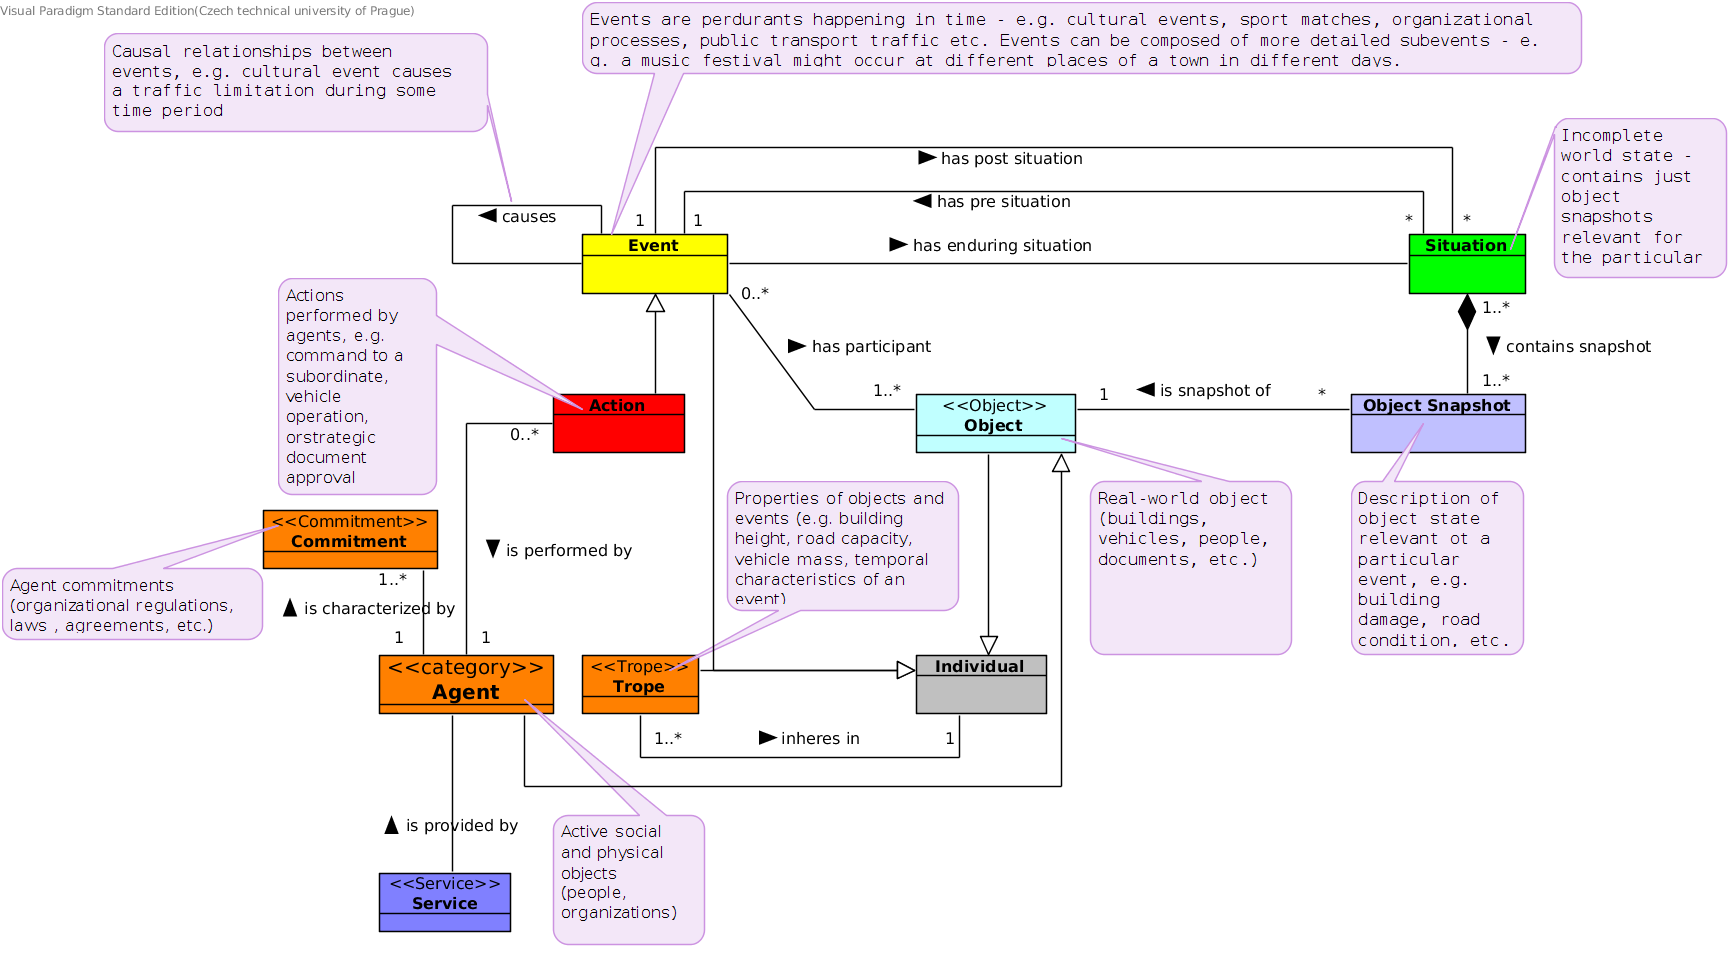
\includegraphics[width=1.0\textwidth]{images/ufo.png}
 \caption{Fundamental concepts and relations of UFO.}\label{fig:ufo}
\end{figure}

\subsubsection{OntoUML}\label{sec:oum}

OntoUML is a language provided on top of UFO for the purpose of conceptual modeling. The language is introduced in \cite{g2006ofscm}. We will review the most important notions necessary for the purpose of this paper.
\begin{description}
 \item[Sortal vs. Mixin.] a \emph{Sortal} is any universal carrying a principle of identity, e.g. \emph{Person} universal (identifiable by DNA, or birth number, etc.), contrary to \emph{Mixin} universal, e.g. \emph{Object} universal having different principles of identity given by its sub types - Person, Building, Vehicle, etc. 
 \item[Rigid vs. Anti-rigid.] \emph{Rigid} is any universal, for which all its instances (individuals) belong to the universal for the whole time of their existence, e.g. \emph{Person} sortal universal. \emph{Anti-rigid} is any universal for which all its instances will not be in the future, or were not in the past instances of the universal, e.g. \emph{Moving Vehicle} sortal universal.
 \item[Kinds and subkinds.] a \emph{Kind} is any rigid sortal, that provides principle of identity, e.g \emph{Person} kind, contrary to a \emph{subkind}, any rigid sortal principle of identity of which is inherited from its ancestor \emph{Kind}, e.g. \emph{Man} subkind inherits its identity from the \emph{Person} kind.
 \item[Phase sortals and role sortals.] a \emph{Phase sortal} is an anti-rigid sortal for which intrinsic properties of an individual are those that make the individual an instance of that anti-rigid sortal, e.g. being a \emph{Teenager} depends on the age of the particular person. In contrast, a \emph{Role sortal} is an anti-rigid sortal for which relation with another individual makes the particular individual an instance of that anti-rigid sortal, e.g. being a \emph{School building} depends on the use of the particular building.
 \item[Relators and relations.] A \emph{Relator} reifies the notion of a relation among several individuals, e.g. \emph{Construction} (as a relation between a company, a building, etc. existing during the \emph{Construction} event in given time frame).
 \item[Powertypes.] A powertype represents the notion of a \emph{type of types} introduced and analysed in~\cite{gpagc2015toap}.
 Powertypes is a fundamental notion for product type modeling (like \emph{building type}), or social role modeling (like \emph{Urban planning expert type}).
\end{description} 
 
\section{Urban Planning Ontology}\label{sec:ontology}

The whole process of ontology modelling has been conducted for over ten months and can be separated in several phases. In the first phase, ontology designers became familiar with data published IPR and chose the adequate ontology modeling technique. In the second phase, ontology model prototypes based on the basic knowledge of data were created and consulted with data professionals employed by IPR. They have provided information and annotations of five thematically similar datasets. Third phase of design started with ontological modelling of datasets. Because of terminology ambiguities, most of the notions are contextualized Data are put in contexts and therefore, single ontologies for every context were created.

% co jsme dostali od IPR,

\subsection{Data analysis}\label{sec:analysis}
Prague Institute of Planning and Development manages tens of datasets, publishing them as open data on their open data geoportal. Datasets contain data related to the city management, urban planning data, data about traffic, POIs and more. For the publication, standardised ATOM service is used. All data sets shall be provided with metadata according to the ISO 19115\cite{ISO19115}. Data are discovered on the geoportal as well, by the keywords. Set of keywords, including names of spatial objects, their attributes and words used for searching data by users themselves, was provided by IPR. The list contains more than 200 keywords with different meanings. Some of the concepts are used in various meanings, some concepts have the same meaning as another, e.g. \texttt{park and ride}, \texttt{Park \& ride} and \texttt{P + R}. Some concepts may have different meaning in different contexts, e.g. \emph{construction} and \emph{building} may have similar or same meaning in the context of the Land use dataset, but in the context of the Buildings dataset, \emph{building} is a specialization\cite{} of a \emph{construction}, i.e. every \emph{building} is a \emph{construction} and all properties of a \emph{construction} are properties of a \emph{building} as well. Moreover, concept of \emph{construction} can be used in the meaning of a process or an object. Context differs among datasets, specific groups of users, object or attribute type and more.

% první zpracování modelů,
First task was to sort concepts, find one common theme and try to find relations between concepts related to the chosen theme. According to the first look on the set of concept, traffic seemed to be suitable theme to start with. First conceptual model was created on the basis of railway traffic. For the first model, mainly specializations were used and only few object properties. Fourteen concepts related to the railway were derived from the set and the contexts and relations were searched for among them. For example, concepts \emph{railway}, \emph{road} and \emph{rail crossing} are definitely somehow related. Relations between objects are ambiguous and for the person without any knowledge and expectations, it is quite difficult to discover such ambiguities. In the example above, \emph{crossing} may be part of \emph{railway}, but also, it may be the part of \emph{road}. \emph{Road} and \emph{railway} may touch, but their connection may be done only in \emph{crossing}. In some cases, \emph{railway} could have been removed, but \emph{crossing} is still on its place. Inexperienced mind also tends to think about same objects in different meanings in different situations. It was proved that the most important thing is to capture meanings for every concept properly and document it (by means of an OWL annotation), and then count every meaning as one object. Therefore it is very important to have at least common knowledge of the topic that is described by the model. 

\begin{figure}
 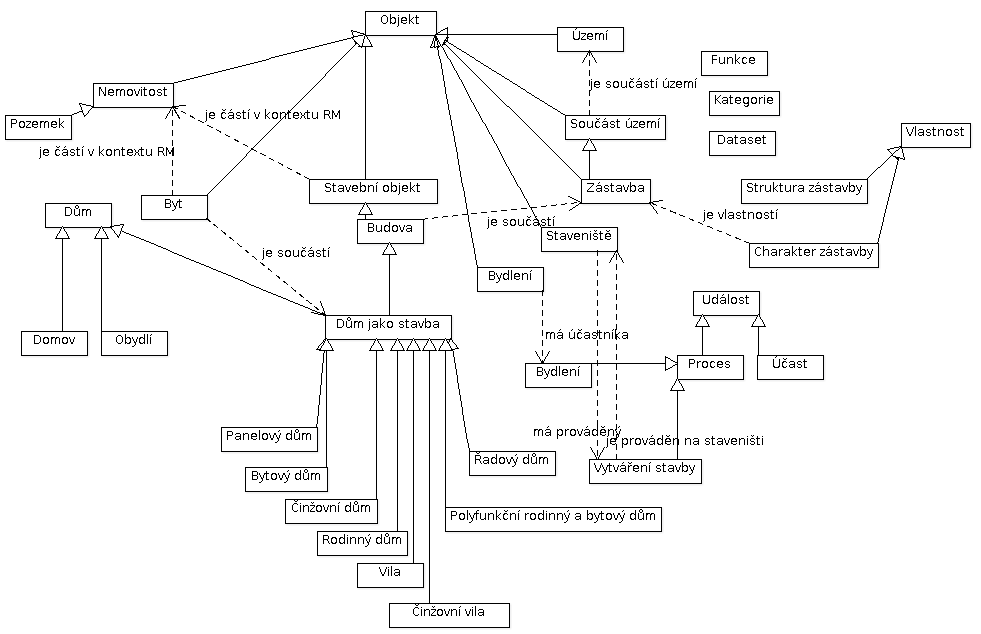
\includegraphics[width=1.0\textwidth]{images/znalostniModel.png}
 \caption{The first semantic model of the ontology created over urban planning data.}\label{fig:model_june}
\end{figure}

The analysis of railway traffic was performed in order to become familiar with the domain and setup basic notions for urban planning. In the next steps we extended the model of traffic in Prague with more interlinked data in order to test the potential to answer distributed queries. The issue of urban planning is still quite wide for the basic model. For this purpose the domain of \emph{housing} was selected by domain experts from IPR.

\subsection{Ontology modelling}\label{sec:modelling}
% přechod na modely územního plánování, 

The first model of urban planning ontology was designed from bottom to the top -- first, basic concepts for the housing issue were derived from the set into the new ontology. Second step was to find and mark relations between objects in the model and important relations heading out of the existing model. Relations and outer objects were added to the model. Besides specializations, object properties starting to be more important in the conceptual model of housing (see Figure \ref{fig:model_june}). Still, every object can be seen in various roles depending on the context. At this stage, the crucial problem was to correctly define meanings (concepts) for different terms in different contexts.

Very important input to the model came from IPR, because the meaning of some concepts were misunderstood. Good example can be the word \emph{real estate}, having different meaning in the context of various groups of users -- for urban planners it is used as \emph{unmovable object, including flats}, for brokers it is \emph{a building or ground, but also a flat or even movable objects such as residential caravans}, and from the perspective of an employee of the cadastral office, \emph{building may be a part of ground and some juridical relations are considered real estates}. These records had to be set straight.

% využití a popis datových sad, včetně obrázků modelů,

\begin{figure}
 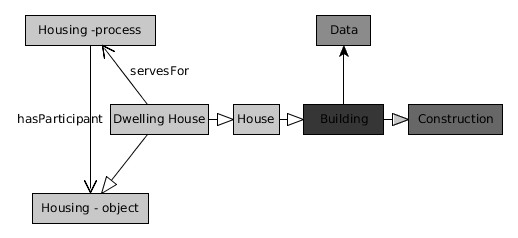
\includegraphics[width=1.0\textwidth]{images/BUILDINGS.png}
 \caption{Model of buildings according to the technical map.}\label{fig:dat_buil}
\end{figure}

At this stage of work, design split into integrated thematic units. Ontology was planned to be used in the context of datasets managed by IPR, therefore it was necessary to understand structure and content of those datasets. As a content of the sample set of datasets, five datasets were chosen:
\begin{description}
 \item[Buildings] is a dataset containing polygons of buildings according to the technical map,
 \item[Floors] is a dataset containing data about buildings with information of their heights and number of floors,
 \item[Current land use] is a dataset containing data describing areas and their parts, their function and form of development in the area,
 \item[Functional land use] is a dataset, that is part of spatial plan, containing data describing designed functional land use,
 \item[Parcels] is a dataset containing data about cadastral parcels.
\end{description}
For each dataset, visual model of relations and involved classes was created. The result is in Figures \ref{fig:dat_buil}, \ref{fig:dat_flo}, \ref{fig:dat_clu}, \ref{fig:dat_fua} and \ref{fig:dat_par}. In the models, the darkness of the class is proportional to the importance of the concept w.r.t. the particular dataset.

\subsubsection{Buildings}

% něco obecně k budovám
In the dataset Buildings there are almost the same information as in the dataset Floors. Differences are in attributes and in the context. Buildings are not in wide context, therefore it is the simplest dataset among the five chosen, at least according to the number of related classes. The main class in the dataset is building, carrying information about it in the form of individuals:
\begin{description}
\item[identifier] is a unique code for every building, 
\item[house number] is identifier of building in a given area,
\item[house number type] is a house type identifier.
\end{description}
Building object also carry information about lifespan and publisher.

\subsubsection{Floors}

% něco obecně k podlažnostem

\begin{figure}
 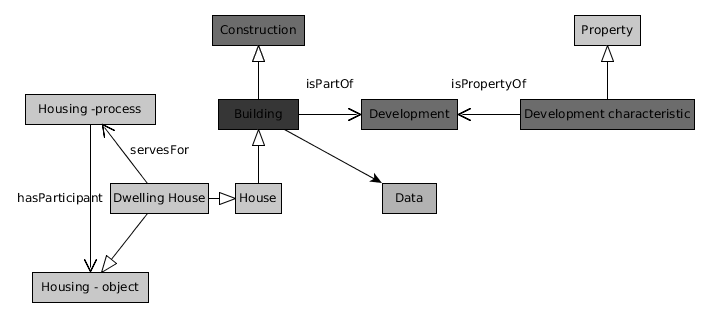
\includegraphics[width=1.0\textwidth]{images/FLOORS.png}
 \caption{Model of buildings and objects relative to them and their properties in the context of floors dataset.}\label{fig:dat_flo}
\end{figure}

Floors shall contain information about heights and shape of buildings. Shape of buildings in the area affects the characteristics of development. Therefore, more classes are possibly related to this theme and model is wider, although it contains information about the same kind of object. Attributes carried by building class are:
\begin{description}
\item[type of object] is the type of building, value itself comes from the codelist,
\item[number of floors] is the sum of floors both above and under ground,
\item[type of roof] defines the shape of roof,
\item[number of roof floors] defines how many floors are narrowed by the roof,
\item[number of floors in the slope] defines how many floors may be partially underground.
\end{description}
Building object also carry information about lifespan and publisher.

\subsubsection{Current land use}

% něco obecně k současnému využití území

\begin{figure}
 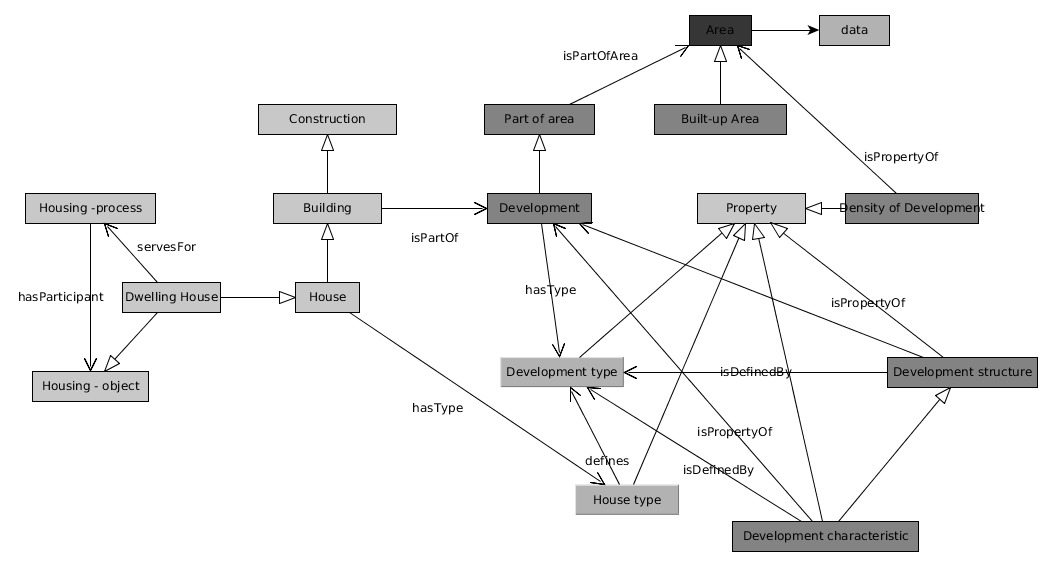
\includegraphics[width=1.0\textwidth]{images/SSVU.png}
 \caption{Model of current land use relative obects and their properties.}\label{fig:dat_clu}
\end{figure}

Information--bearing object is an area. Objects in the context of this datasets carries information about the real land use. It may differ from the planed or purposed land use. Context covers really lot of objects, because current land use is influenced by lot of aspects.

Information carried by area object itself is not so rich:
\begin{description}
\item[land use code] is the information about main current land use, value itself comes from the codelist,
\item[behind Prague] defines, if the area lies within the capital borders, or not,
\item[other use] defines secondary land use, value itself comes from the codelist.
\end{description}
Area object also carries information about publisher.

\subsubsection{Functional land use}

% něco obecně k užití ploch

\begin{figure}
 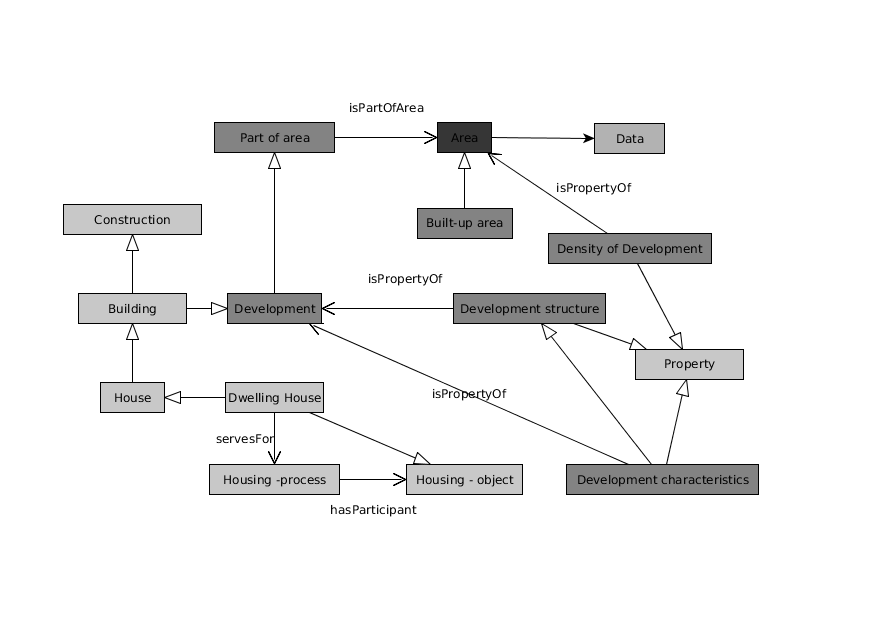
\includegraphics[width=1.0\textwidth]{images/FVU.png}
 \caption{Model of functional land use relative objects and their properties.}\label{fig:dat_fua}
\end{figure}

Information--bearing object in the dataset is an area. In the urban planning, areas have attached proposed usage. Some of areas are not used the way they should according to this information. Part of development characteristic may be the shape of buildings on it as well. Context of relations in this dataset is quite wide -- a lot of properties are influencing the land use, but not as many as in the case of current use. In the planning, not all possibilities are considered. In the design of functional use, two values are filled for each attribute -- one for design horizon and second one as territorial reserve:
\begin{description}
\item[functional use of area code] is the value from codelist describing planned use of the area,
\item[code of the land use rate] is a value from codelist,
\item[number differentiation] is a number from 1 to 7,
\item[composite code] is a text.
\end{description}

\subsubsection{Parcels}

% něco obecně k parcelám

\begin{figure}
 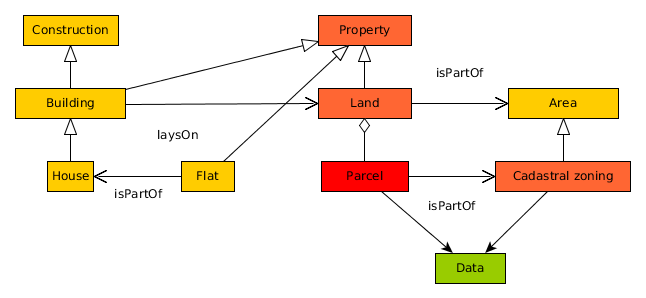
\includegraphics[width=1.0\textwidth]{images/PARCELS.png}
 \caption{Model of cadastral parcels and objects relative to them and their properties in the context of parcels dataset.}\label{fig:dat_par}
\end{figure}

Dataset parcels contains information about cadastral parcels and their affiliation to the cadastral zonings. For the purpose of the model design of this dataset, new class had to be created. The class is called cadastral zoning and in the context of urban planning, its meaning is relevant only for this dataset (as far as is the context of five designed datasets). The main information--bearing class is parcel, but cadastral zoning carries on attribute too. Attributes of parcel are:
\begin{description}
\item[identifier] is a unique code within whole dataset,
\item[parcel number] is the unique identifier within cadastral zoning,
\item[date of creation/last change/deletion] is the par of the objects life cycle,
\item[area] is the acreage of the parcel in square meters.
\end{description}
Cadastral zoning has only one attribute:
\begin{description}
\item[code of the cadastral zoning] is unique identifier of cadastral zoning within whole dataset.
\end{description}

The word \textit{Property} in the context of dataset Parcels has different meaning than \textit{Property} in the context of datasets Current land use and Functional land use. In the previous cases, property is an abstract class pointing to an attribute or feature (e.g. density is property of population). In the context of parcels, property is an object owned or possessed by some entity, private or legal (e.g. building is property). Interesting fact is, that this problem depends on the language used in model. In Czech, two meanings of property are differently named.

% výrazové prostředky definice atributů, individuály

All models, including classes (objects) and properties (relations) were transposed into the ontology. In datasets is a big amount of concepts used in two or more of datasets. Some of them are used in different contexts in every occasion. At this stage, dividing classes into more is not the simplest way of adding context to the ontology. Since the contexts of concepts begun to be more important to the completeness and entirety of the model, more effective way of distinguishing contexts had to be found. It was decided to divide ontologies into more files, according to its context. 

\subsection{Semantic contexts}
% Ontologie jednotlivých datových sad, -- 

For the purposes of this work, context is represented by datasets. For every dataset, a single ontology was created, represented by single file. For every dataset described in \ref{sec:modelling}, new ontology was created. In those ontologies are held only the properties, classes and individuals related to the context of dataset. Classes and properties having the same ontological meaning in every use are stored in the ontology \textit{common}. The rest of the concepts, that were not used in any of datasets were moved to the ontology \textit{appendix}. In the ontology common, only common objects and relations are visible. In ontologies representing dataset contexts, all content from \textit{common} ontology are visible as well. For the better information about context of dataset, every class, individual and property is annotated as \textit{isInContextOfDataset}. For the visualisation and querying over the whole urban planning ontology, ontology \textit{all} was created. Summary of ontologies and relations among them is shown in the Figure \ref{fig:ontologies_summary}. Some of the properties may be used in the same context even in more than one ontology. For these cases, more ontologies can be created and then imported into all applicable ontologies (bright blue).

\begin{figure}
 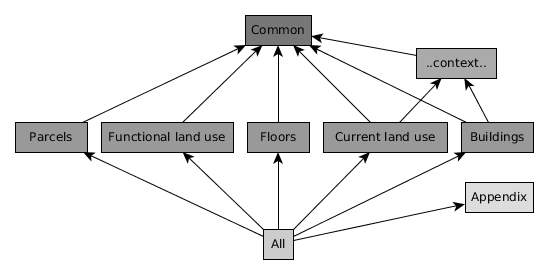
\includegraphics[width=1.0\textwidth]{images/ontologies.png}
 \caption{Summary of dataset ontologies and relations among them.}\label{fig:ontologies_summary}
\end{figure}

Context itself is defined as a class in the \textit{common} ontology as a specialization of information object. Possibility of adding new types of context in the future remains open, therefore  the structure of information objects remains more branched, than needed on the first sight.

\section{Practical Queries and Evaluation}\label{sec:eval}

% uvaha o dotazopvaci strukture (obrázek schématu)
The purpose of ontology model is to get rich linked information from the datasets. One of the proposed targets is creation of a querying mechanism over the IPR datasets on their geoportal. Their idea is querying mechanism, that returns not only exact matches, but rates related responses and returns matches, that may have something in common. Problem of browsing data by users is, by the words of IPR, that users do not know, what exactly do they expect. It is quite import to know, what kind of queries IPR expects to be asked. They have provided us with following examples:
\begin{enumerate}
\item What areas shall be used for housing according to the spatial plan, but their current use is different and are owned by municipality?
\item In which areas lie apartment houses taller than four floors?
\item How many percent of the floor area in the Old Town is used for housing?
\item How many family houses are in Uh{\v r}{\' i}n{\v e}ves?
\item Which office buildings have no parks in their neighbourhood?
\item What is the floor area of all office buildings in Prague?
\item Which gas stations lie in areas, where no gas stations shall lie?
\item In which municipal areas are tenement houses?
\item Which buildings in proximity of given point are owned by public subjects and are able to be used for the building of new library?
\end{enumerate}
\begin{figure}
 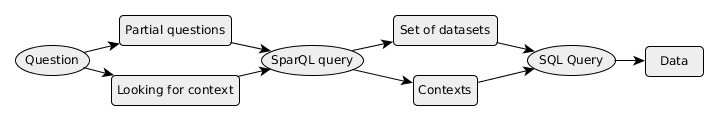
\includegraphics[width=1.0\textwidth]{images/querying.png}
 \caption{Process of asking question over the ontology and datasets.}\label{fig:querying}
\end{figure}
All of these questions are quite complex and lot of them may be answered in different ways. All of these questions are querying data itself. Data are not part of ontology model. Moreover, some concepts are not clear in its meaning, e.g. Uh{\v r}{\' i}n{\v e}ves can be a name of part of municipality or cadastral zoning. Another question is on the meaning of words like ``neighbourhood'', ``shall'', ``used for'' and similar. Good example of many meanings in one question is number eight: In which municipal areas are tenement houses? Municipal area may be administrative unit of municipality, but it also may be an area inside municipality or area of parcels, on which is urban area. Second part of the question is problematic as well. Answer may refer to houses with the type ``tenement'', or houses in areas with attribute ``used for tenement''. Each question shall be divided into elements and for this elements context (or more possible contexts) shall be found. For the search, ontology querying shall be used.
% dotazy na strukturu a kontext -- SparQL

For the querying the context and structure of contents used in question is used SparQL language. Queries are applied upon the \textit{all} ontology, that contain all information about datasets, including context. Questions above could be split into set of SparQL queries defining context and datasets, where to look for information. The result of SparQL shall be the set of datasets and classes in specific context, relevant for finding the answer on asked question.

Basic set of SparQL queries shall provide answer on following questions:
\begin{enumerate}
\item in which datasets can be found given concept?
\item in which context is concept used over the set of datasets? 
\item in which dataset can be given found attribute value?
\item what properties are there between two concepts in a given set of datasets?
\item which datasets contain information needed to answer question on specific data?
\end{enumerate}

As seen before, first four questions are basically subsets of the fifth. Question number five is the most important question and in the practical use it shall be used for searching context for further SQL query focused on direct access to data. 

The process of querying proceeds as follows (see Figure \ref{fig:querying}):
\begin{enumerate}
\item User asks a question on the IPR geoportal (that will be probably provided by the third party of the project, private company Gisat), 
\item question is split into parts,
\item context of single parts is queried by SparQL queries,
\item output for the queries is usage and meaning of concepts in proposed context, including datasets and their structures, where specific data can be found,
\item based on the context, SQL queries are created and commited (this will be provided by Gisat).
\end{enumerate}

\section{Conclusions}

In the first year of project, most of the work was done on the ontological models. In the beginning, it was important to get used to the structure and meaning of data and nomenclature used in the field of urban planning. After the first tries of creating ontologies, few specifics were found. It is very important to not underestimate annotations of classes and properties. As the time passes and the number of concepts raises, more and more properties depends on context. 

\subsubsection*{Acknowledgements}\label{sec:ack}
\noindent This work was supported by the grant No. TA04021499 ``Open Data and semantic approaches to uncover social aspects of urban quality'' of the Technology Agency of the Czech Republic.

% + REFERENCES
\bibliography{16eswc-gison.bib}
\bibliographystyle{unsrt}
\end{document}